\documentclass{article}

% If you're new to LaTeX, here's some short tutorials:
% https://www.overleaf.com/learn/latex/Learn_LaTeX_in_30_minutes
% https://en.wikibooks.org/wiki/LaTeX/Basics

% Formatting
\usepackage[utf8]{inputenc}
\usepackage[margin=1in]{geometry}
\usepackage[titletoc,title]{appendix}

% Math
% https://www.overleaf.com/learn/latex/Mathematical_expressions
% https://en.wikibooks.org/wiki/LaTeX/Mathematics
\usepackage{amsmath,amsfonts,amssymb,mathtools}

% Images
% https://www.overleaf.com/learn/latex/Inserting_Images
% https://en.wikibooks.org/wiki/LaTeX/Floats,_Figures_and_Captions
\usepackage{graphicx,float}

% Tables
% https://www.overleaf.com/learn/latex/Tables
% https://en.wikibooks.org/wiki/LaTeX/Tables

% Algorithms
% https://www.overleaf.com/learn/latex/algorithms
% https://en.wikibooks.org/wiki/LaTeX/Algorithms
\usepackage[ruled,vlined]{algorithm2e}
\usepackage{algorithmic}

% Code syntax highlighting
% https://www.overleaf.com/learn/latex/Code_Highlighting_with_minted
\usepackage{minted}
\usemintedstyle{borland}

% References
% https://www.overleaf.com/learn/latex/Bibliography_management_in_LaTeX
% https://en.wikibooks.org/wiki/LaTeX/Bibliography_Management
\usepackage{biblatex}
\addbibresource{references.bib}

% Title content
\title{AMATH 582 Homework 1}
\author{Daniel Burnham}
\date{January 24, 2020}

\begin{document}

\maketitle

% Abstract
\begin{abstract}
The work presented here is motivated by material covered in AMATH 582 Computational Methods For Data Analysis regarding Fourier transform. The premise of the exercise is that a dog swallowed a marble and the veterinarian collected ultrasound measurements of the marble in the intestines. However, the data needs to be filtered and subsequently analyzed in order to determine where to focus an intense acoustic wave to break apart the marble. Averaging of the data transformed in the frequency domain using the Fourier transform will be used to identify the marble frequency signature. This signature will then be used to locate the marble at each point in time within the data by informing the location of a filter in the frequency domain. After this filtering the marble trajectory will be made clear, and the acoustic wave target can be acquired.
\end{abstract}

% Introduction and Overview
\section{Introduction and Overview}
The data analysis efforts will be divided into three distinct phases. First, the center frequency corresponding to the marble in the Fourier transformed data will be identified. Second, the center frequency will be used to filter the Fourier transformed data for each measurement instance. Third, this filtered data will be inverse transformed to yield the spatial location of the marble for each moment in time.

% data averaging and frequency signature Subsection
\subsection{Marble Frequency Signature}
The frequency signature of the marble will be isolated from the spatial data by first transforming the data into the frequency domain and then averaging the measurements together to diminish noise.

% data filtering subsection
\subsection{Data Filtering}
The center frequency of the marble will be used to position a filter in the frequency domain to isolate the marble signature for each measurement. This filtered frequency spectrum can then be inverse transformed to indicate the spatial location of the marble.

% data filtering subsection
\subsection{Marble Location}
The maximum value of the filtered and subsequently inverse transformed data for each measurement will indicate where the marble is located in space. The visualization of this location for each measurement instance will illustrate the trajectory of the marble in time and will allow for the acoustic wave to be targeted to the final marble position.

%  Theoretical Background
\section{Theoretical Background}
The main concept explored with this work is the Fourier transform. The Fourier transform is an extension of the Fourier series which represents a given function $f(x)$ as sums of cosines and sines. 
\begin{equation}
    f(x) = \frac{a_0}{2} + \sum_{i=1}^\infty \left(a_n\cos{nx} + b_n\sin{nx}\right) \quad x \in (-\pi,\pi].
    \label{eqn:fourierseries}
\end{equation}
This operation is especially useful in the context of signal analysis as it represents signal component frequencies for selective filtering.

To implement the Fourier transform computationally, the fft(x) function in MATLAB will be used. There are certain properties of the fft(x) function that need to be considered. First, the function is only "fast" when passed data that is $2^{n}$ discretized. Second, the algorithm shifts the data so that $x \in [0, L] \rightarrow [−L, 0]$ and $x \in [−L, 0] \rightarrow [0, L]$. Third, a $2\pi$  periodic domain is assumed.

% Algorithm Implementation and Development
\section{Algorithm Implementation and Development}
The main steps of the algorim are as follows: 
\begin{enumerate}
    \item Average frequency spectrum of each measurement instance to identify center frequency of marble.
    \item Filter data in the frequency domain around marble frequency signature. Inverse transform data to find marble trajectory and final position.
\end{enumerate}

\begin{algorithm}
\begin{algorithmic}
    \STATE{Import data from \texttt{Testdata.mat}}
    \FOR{$j = 1:20$}
        \STATE{Extract measurement $j$ from \texttt{Undata}}
        \STATE{Apply Fourier transform}
        \STATE{Add to sum of transformed data}
    \ENDFOR
    \STATE{Divide sum of transformed data by number of measurements}
    \STATE{Find maximum value of the average transformed data}
    
\end{algorithmic}
\caption{Find center frequency}
\label{alg:Marble Frequency}
\end{algorithm}

\begin{algorithm}
\begin{algorithmic}
    \STATE{Create filter around marble frequency}
    \FOR{$j = 1:20$}
        \STATE{Apply filter to each measurement}
        \STATE{Apply inverse transform}
        \STATE{Find maximum value corresponding to the marble position at that time step.}
    \ENDFOR
    \STATE{Visualize trajectory}
    \STATE{Find final marble position}
\end{algorithmic}
\caption{Filter Data}
\label{alg:Filter Data}
\end{algorithm}

% Computational Results
\section{Computational Results}
See Figure~\ref{fig:marbleSignal} for the result of averaging the Fourier transformed measurements. See Figure~\ref{fig:marbleTrajectory} for the determined marble trajectory. The final marble position was determined to be $(-5.6250,       4.2188,   -6.0938)$ in the spatial domain.

% begin{figure}[tb] % t = top, b = bottom, etc.
\begin{figure}
    \centering
    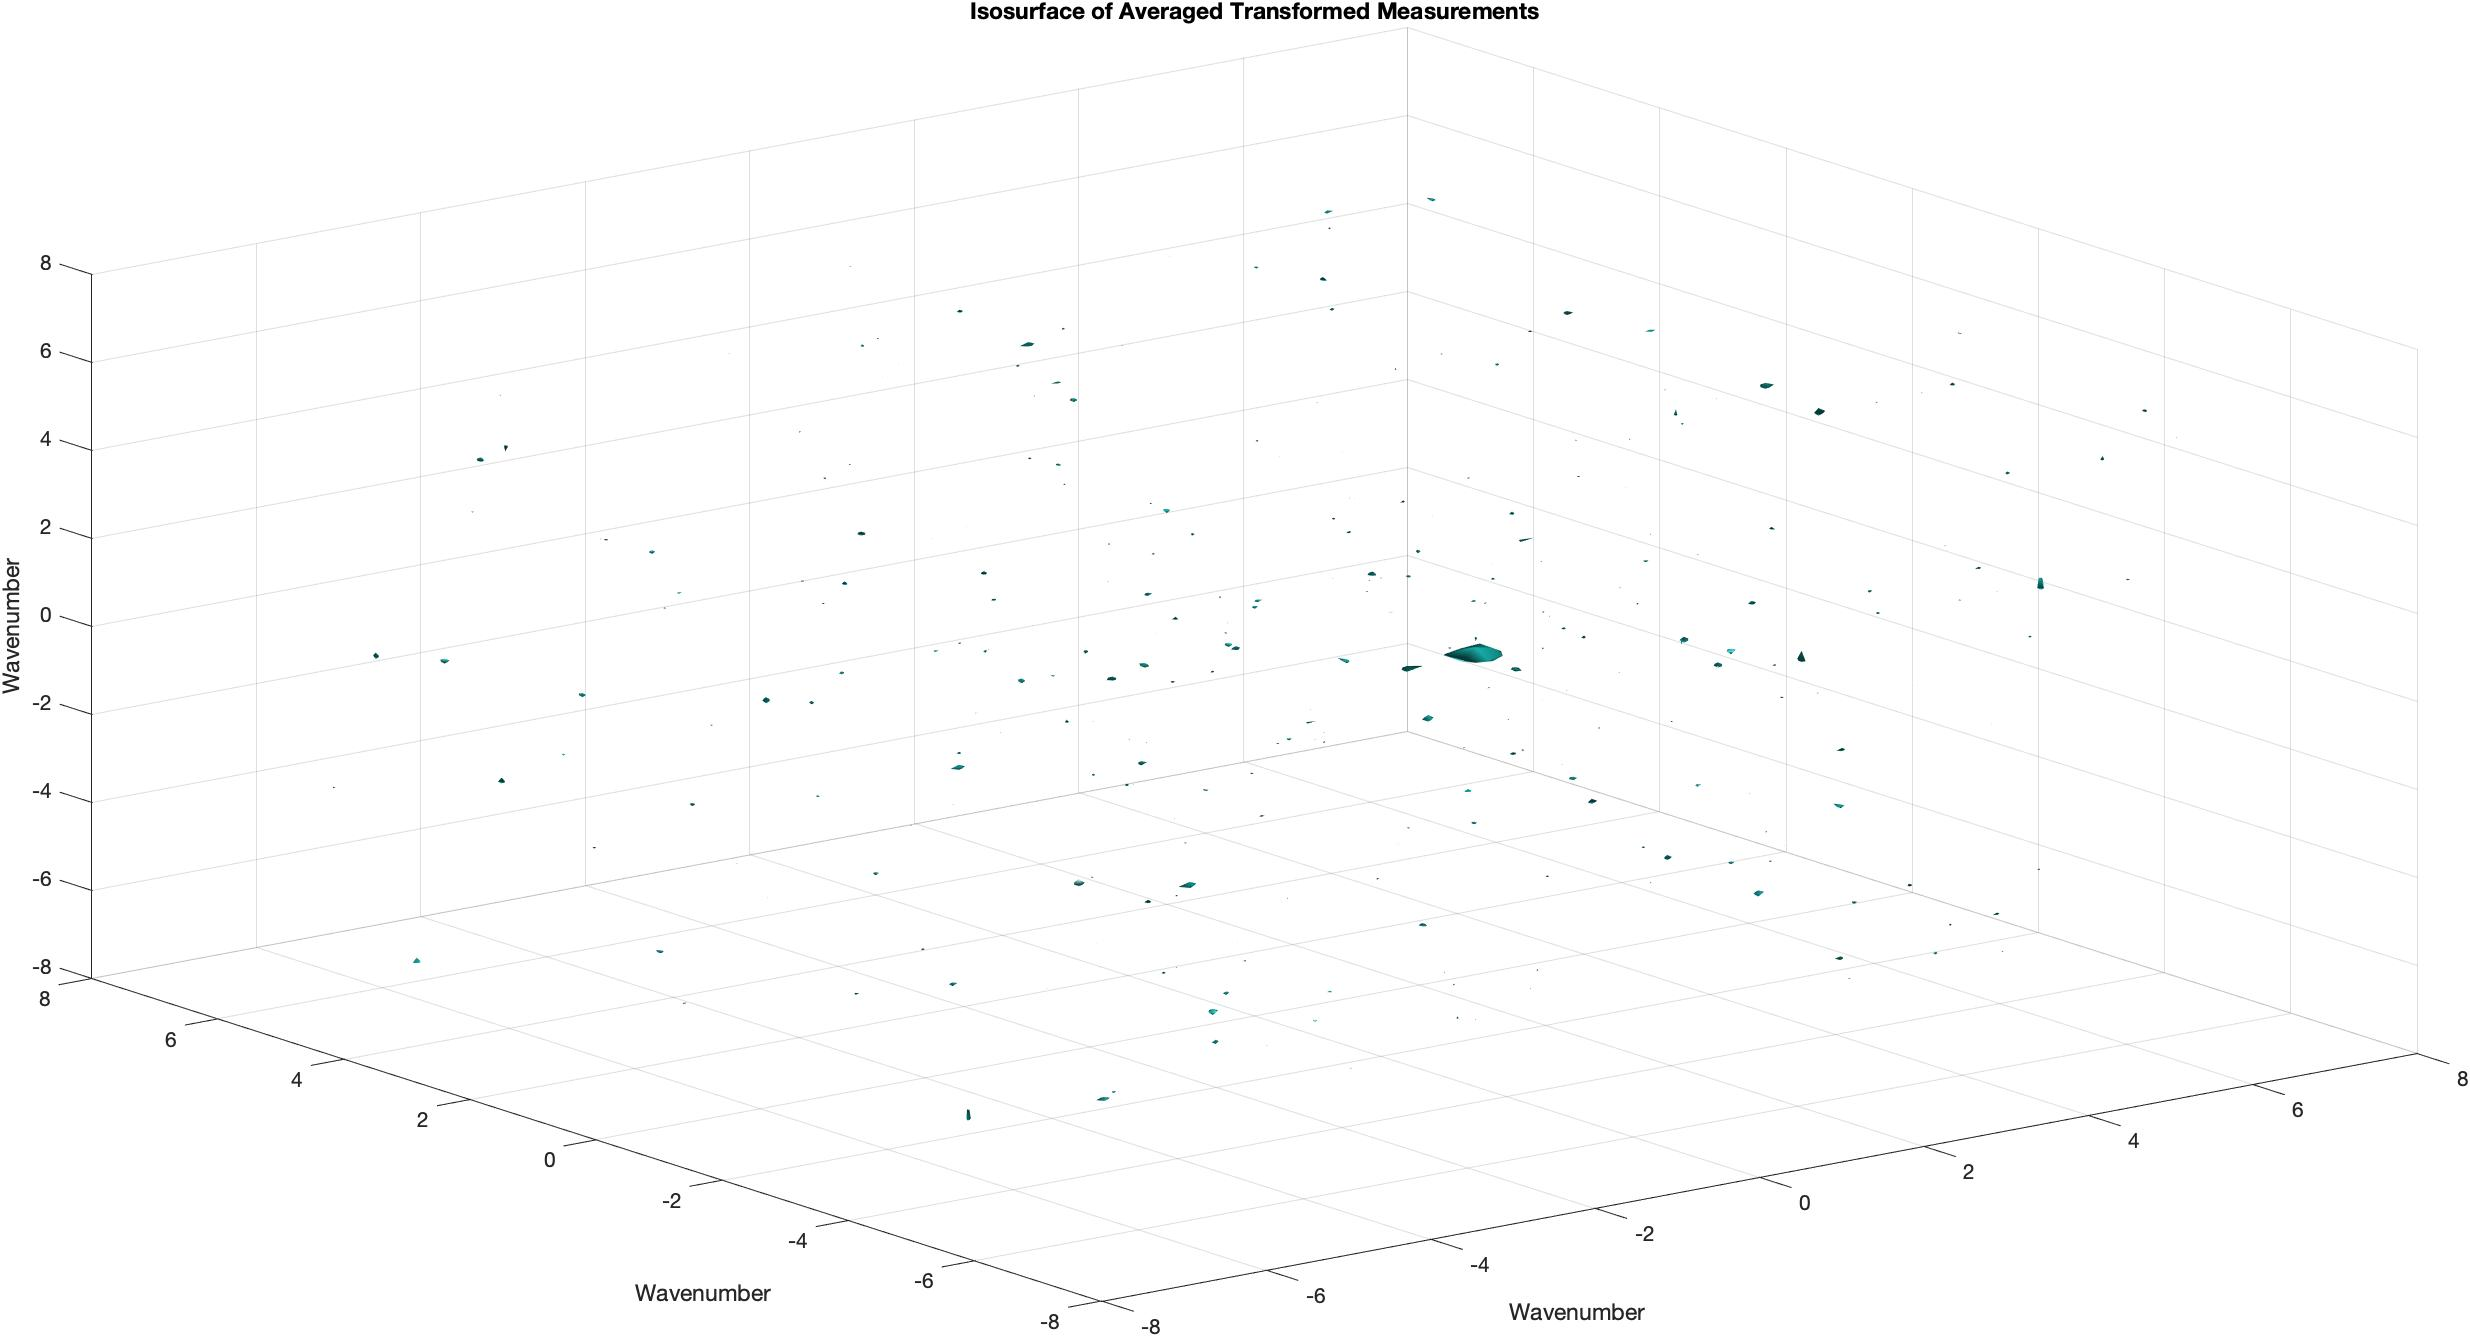
\includegraphics[width=1.0\linewidth]{marbleSignal.jpg}
    \caption{This is an isosurface plot (see Appendix~\ref{itemize:functions}) of the marble central frequency after averaging measurements in the frequency domain. The frequency signature of the marble is $(1.8850, -1.0472, 0)$}
    \label{fig:marbleSignal}
\end{figure}

% begin{figure}[tb] % t = top, b = bottom, etc.
\begin{figure}
    \centering
    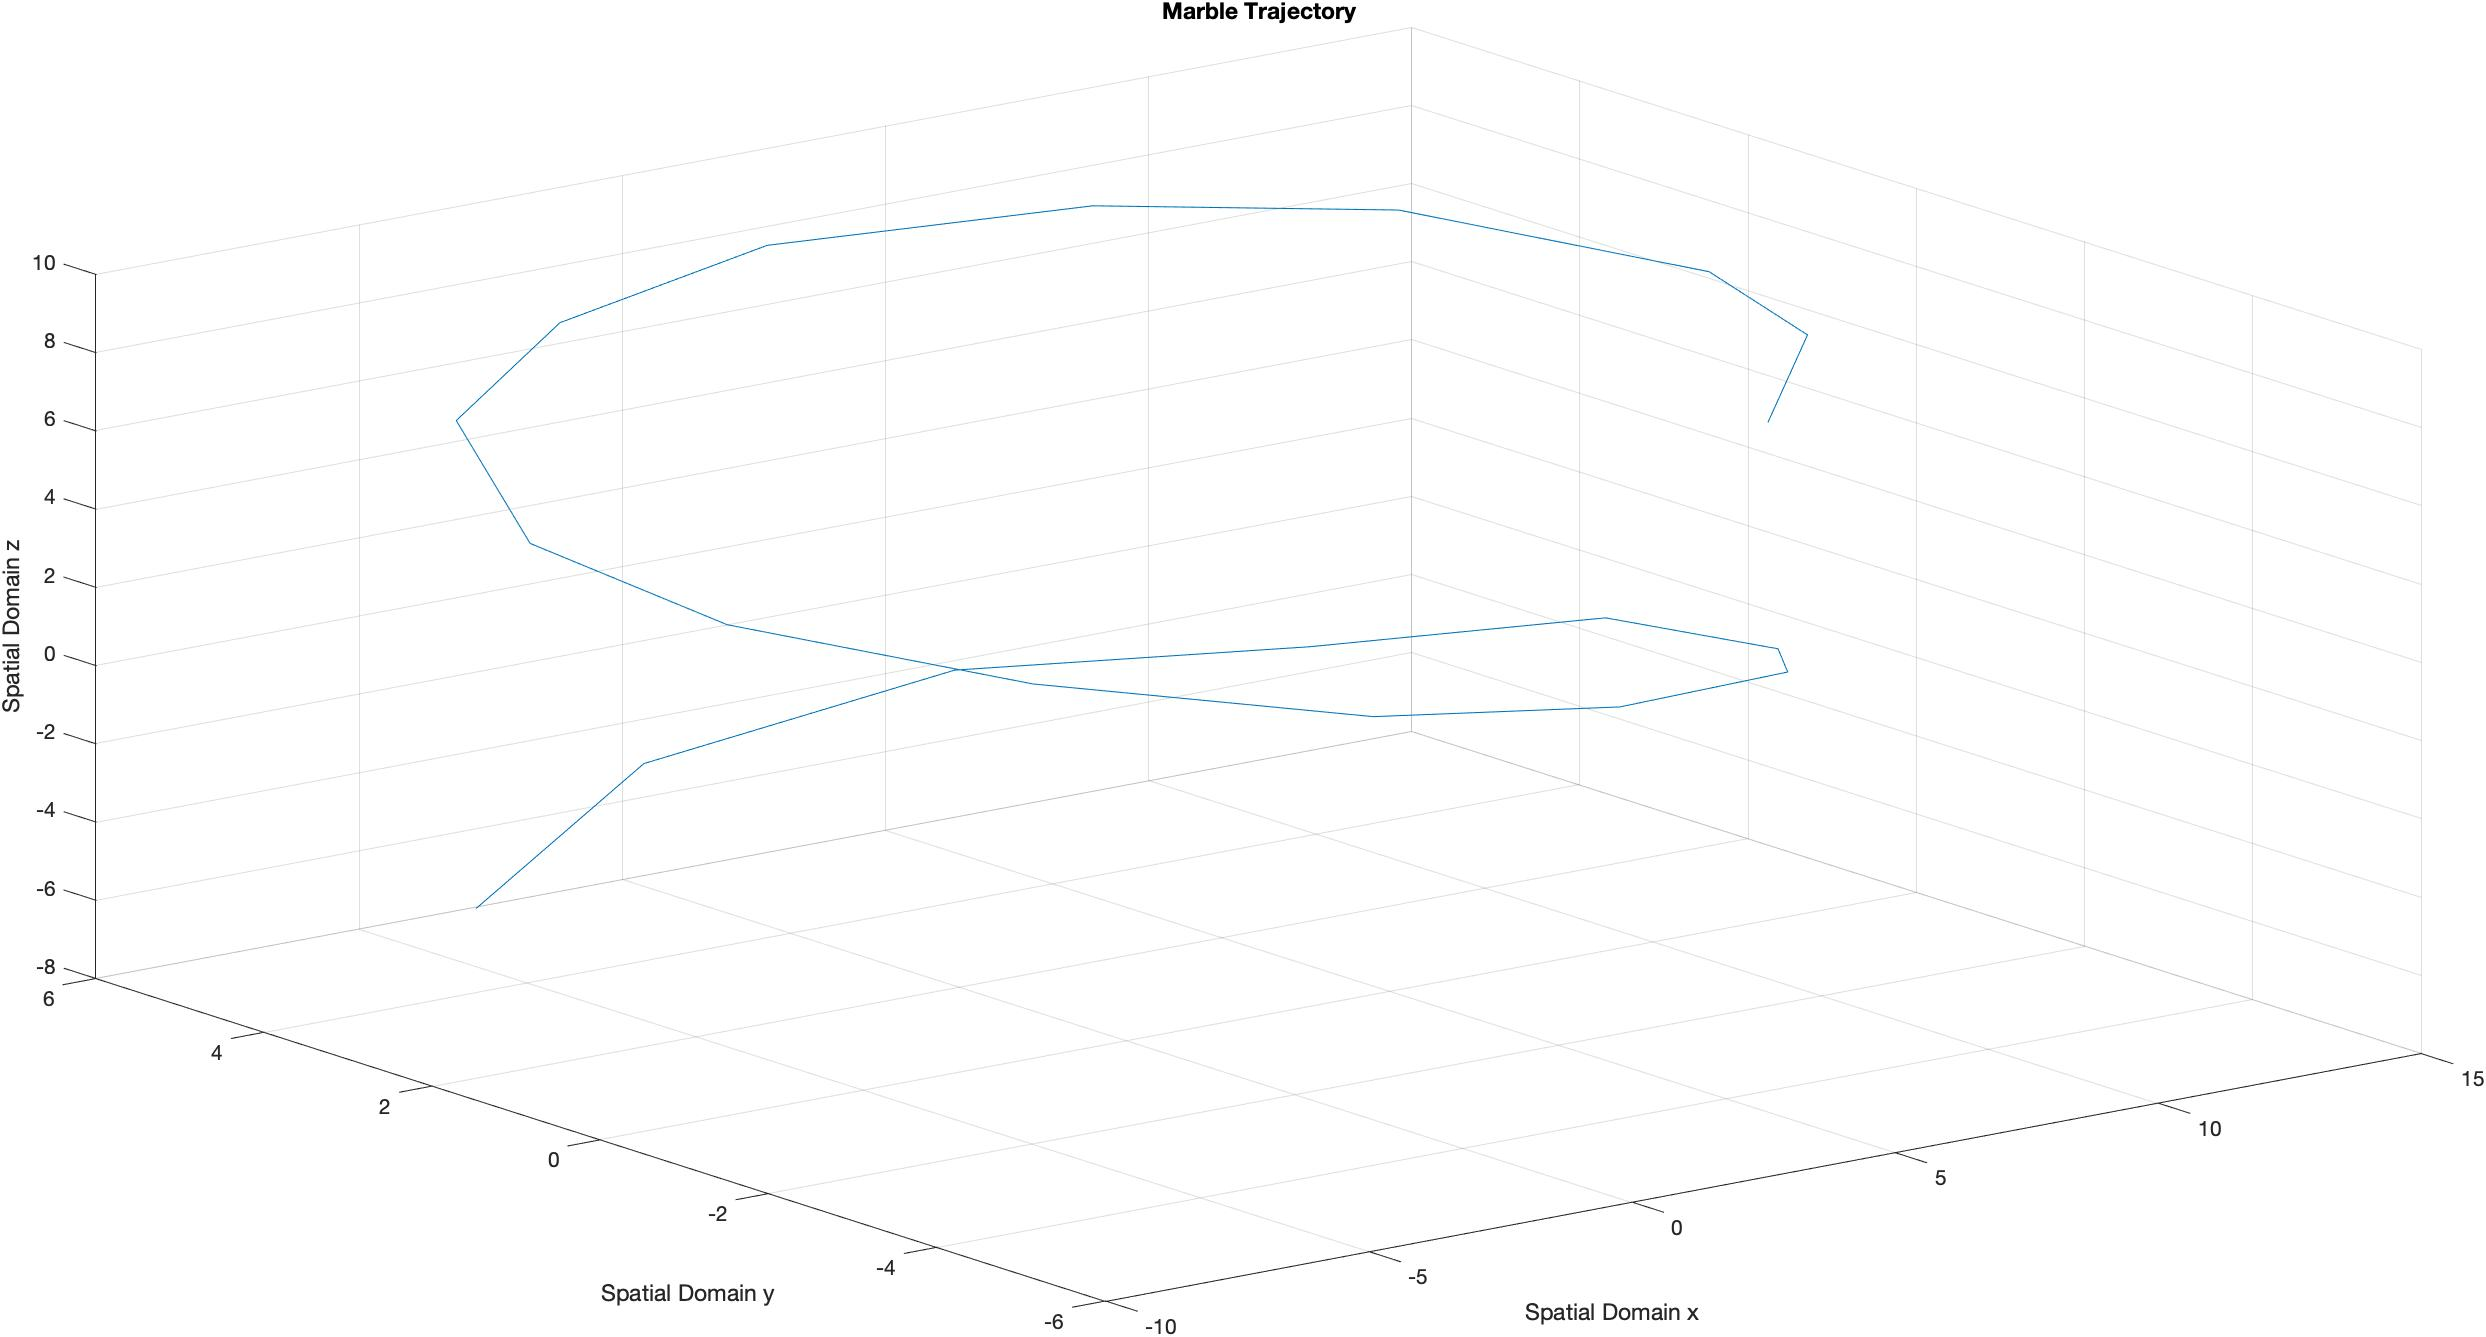
\includegraphics[width=1.0\linewidth]{marbleTrajectory.jpg}
    \caption{This is a 3D plot of the marble trajectory after filtering the data around the central frequency and using the inverse transform. The final marble position is $(-5.6250,4.2188,-6.0938)$ }
    \label{fig:marbleTrajectory}
\end{figure}

% Summary and Conclusions
\section{Summary and Conclusions}
The averaging of the transformed ultrasound measurements successfully diminished the noise in the signal and allowed for the marble frequency signature to be identified. Inverse transformation of the data filtered around this frequency resulted in a spiraling marble trajectory.

% Appendices
\begin{appendices}

% MATLAB Functions
\section{MATLAB Functions}
\begin{itemize}
    \item \texttt{Y = fftn(X)} returns the multidimensional Fourier transform of an N-D array using a fast Fourier transform algorithm. The N-D transform is equivalent to computing the 1-D transform along each dimension of X. The output Y is the same size as X.
    \item \texttt{Y = fftshift(X)} rearranges a Fourier transform X by shifting the zero-frequency component to the center of the array.
    \item \texttt{X = ifftn(Y)} returns the multidimensional discrete inverse Fourier transform of an N-D array using a fast Fourier transform algorithm. The N-D inverse transform is equivalent to computing the 1-D inverse transform along each dimension of Y. The output X is the same size as Y.
    \item \texttt{[row,col] = ind2sub(sz,ind)} returns the arrays row and col containing the equivalent row and column subscripts corresponding to the linear indices ind for a matrix of size sz. Here sz is a vector with two elements, where sz(1) specifies the number of rows and sz(2) specifies the number of columns.
    \item \texttt{fv = isosurface(X,Y,Z,V,isovalue)} computes isosurface data from the volume data V at the isosurface value specified in isovalue. That is, the isosurface connects points that have the specified value much the way contour lines connect points of equal elevation.
    \item \texttt{[X,Y] = meshgrid(x,y)} returns 2-D grid coordinates based on the coordinates contained in the vectors \texttt{x} and \texttt{y}. \text{X} is a matrix where each row is a copy of \texttt{x}, and \texttt{Y} is a matrix where each column is a copy of \texttt{y}. The grid represented by the coordinates \texttt{X} and \texttt{Y} has \texttt{length(y)} rows and \texttt{length(x)} columns. 
\label{itemize:functions}
\end{itemize}

% MATLAB Codes
\section{MATLAB Code}
\begin{listing}[h]
\inputminted{matlab}{HW1_DanielBurnham.m}
\caption{MATLAB code from external file used to generate the results presented here.}
\label{listing:HW1code}
\end{listing}

\end{appendices}

\end{document}
